\documentclass[10pt]{beamer}

% Língua e acentos
\usepackage[brazil]{babel}
%\usepackage[utf8]{inputenc}
%\usepackage[T1]{fontenc}

% Tema
\usetheme{metropolis}
\usepackage{appendixnumberbeamer}
\usepackage{booktabs}
\usepackage[scale=2]{ccicons}
\usepackage{pgfplots}
\usepackage{xspace}

\newcommand{\themename}{\textbf{\textsc{metropolis}}\xspace}


\title{Análise de artigo científico}
\subtitle{\textit{Video object tracking using adaptive Kalman filter}}
\date{\today}
\author{David Maykon Krepsky Silva}
\institute{Departamento de Computação - Mestrado - UEL}
\titlegraphic{
\includegraphics[height=1.2cm]{images/logo-dc.png}\hfill
\includegraphics[height=1.0cm]{images/logo.jpg}}

\begin{document}

\maketitle

\begin{frame}{Sumário}
  \setbeamertemplate{section in toc}[sections numbered]
  \tableofcontents[hideallsubsections]
\end{frame}

\section{Introdução}
%%%%%%%%%%%%%%%%%%%%%%%%%%%%%%%%%%%%%%%%%%%%%%%%%%%%%%%%%%%%%%%%%%%%%%%%%%%%%%%%
% Segmentação de objetos em vídeo
%%%%%%%%%%%%%%%%%%%%%%%%%%%%%%%%%%%%%%%%%%%%%%%%%%%%%%%%%%%%%%%%%%%%%%%%%%%%%%%%
\begin{frame}{Segmentação de objetos em vídeo}
Uma aplicação real que utiliza a segmentação de objetos em vídeo é composta por três partes \cite{Weng2006}:

\begin{enumerate}
	\item problema inicial da segmentação de objetos em movimento; %after effects
	
	\item detecção do objeto em movimento;
	
	\item acompanhamento (rastreio) do objeto em movimento.
\end{enumerate}
\end{frame}
%%%%%%%%%%%%%%%%%%%%%%%%%%%%%%%%%%%%%%%%%%%%%%%%%%%%%%%%%%%%%%%%%%%%%%%%%%%%%%%%
% Definição do Problema
%%%%%%%%%%%%%%%%%%%%%%%%%%%%%%%%%%%%%%%%%%%%%%%%%%%%%%%%%%%%%%%%%%%%%%%%%%%%%%%%
\begin{frame}[fragile]{Definição do problema}
	Problemas encontrados na segmentação de vídeo:
	
 	\begin{description}
		\item[Oclusão] o objeto desaparece total ou parcialmente;
		
		\item[Direção] mudanças abruptas na direção ou sentido;
			
		\item[Iluminação] sombras, reflexos ou variação da luz durante o vídeo;
		
		\item[Velocidade] objetos que se movem muito rápido ou que possuem grande aceleração.
	\end{description}
\end{frame}

\begin{frame}[fragile]{Definição do problema}
  \begin{figure}[H]
  	\label{fig:conventional-alg}
  	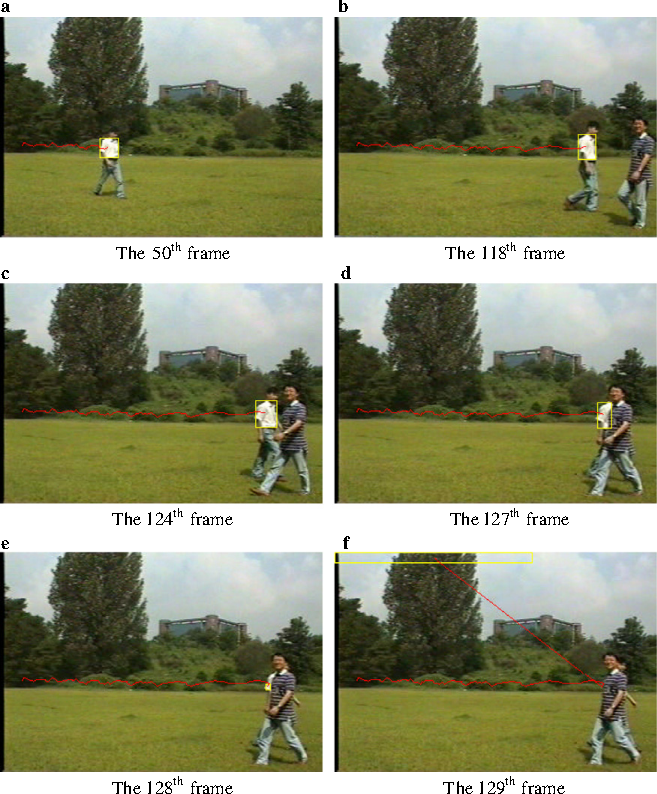
\includegraphics[scale=0.45]{images/fig1.pdf}
  	\caption{Experimento utilizando algoritmo de rastreamento convencional. Fonte: Weng, S. K. \textit{et al.}, 2016.}
  \end{figure}
\end{frame}

%%%%%%%%%%%%%%%%%%%%%%%%%%%%%%%%%%%%%%%%%%%%%%%%%%%%%%%%%%%%%%%%%%%%%%%%%%%%%%%%
% Objetivo do artigo
%%%%%%%%%%%%%%%%%%%%%%%%%%%%%%%%%%%%%%%%%%%%%%%%%%%%%%%%%%%%%%%%%%%%%%%%%%%%%%%%
\begin{frame}[fragile]{Objetivo do artigo}
	\begin{center}
		\alert{O objetivo do artigo é a elaboração de um algoritmo eficiente para rastreamento de objetos em vídeo.}
	\end{center}
\end{frame}

%%%%%%%%%%%%%%%%%%%%%%%%%%%%%%%%%%%%%%%%%%%%%%%%%%%%%%%%%%%%%%%%%%%%%%%%%%%%%%%%
% Aplicações
%%%%%%%%%%%%%%%%%%%%%%%%%%%%%%%%%%%%%%%%%%%%%%%%%%%%%%%%%%%%%%%%%%%%%%%%%%%%%%%%
\begin{frame}[fragile]{Aplicações}
Possíveis aplicações do algoritmo:

\begin{itemize}
	\item monitoramento e segurança;
	\item análise de esportes;
	\item anotações em vídeo;
	\item controle de tráfego;
	\item dentre outras.
\end{itemize}
\end{frame}

%%%%%%%%%%%%%%%%%%%%%%%%%%%%%%%%%%%%%%%%%%%%%%%%%%%%%%%%%%%%%%%%%%%%%%%%%%%%%%%%
% Solução proposta
%%%%%%%%%%%%%%%%%%%%%%%%%%%%%%%%%%%%%%%%%%%%%%%%%%%%%%%%%%%%%%%%%%%%%%%%%%%%%%%%
\begin{frame}[fragile]{Solução proposta}
\begin{center}
	Utilizar o \textbf{Filtro de Kalman} para estimar a posição do objeto de interesse.
\end{center}
\end{frame}

\section{Filtro de Kalman}

%%%%%%%%%%%%%%%%%%%%%%%%%%%%%%%%%%%%%%%%%%%%%%%%%%%%%%%%%%%%%%%%%%%%%%%%%%%%%%%%
% Filtro de Kalman
%%%%%%%%%%%%%%%%%%%%%%%%%%%%%%%%%%%%%%%%%%%%%%%%%%%%%%%%%%%%%%%%%%%%%%%%%%%%%%%%
\begin{frame}{Definição}
	O Filtro de Kalman é um estimador de estado ótimo, o qual infere o valor de uma variável a partir de medidas indiretas que possuem um certo grau de incerteza \cite{Faragher2012}.
\end{frame}

\begin{frame}{Definições}
	Se a incerteza presente nas amostras for Gaussiana, o filtro de Kalman minimiza	o valor do erro quadrático médio do parâmetro estimado.
	
	Se o ruído não for Gaussiano, o filtro de Kalman é o melhor estimador linear possível \cite{Kleeman}.
\end{frame}

\begin{frame}{Diagrama de blocos}
\begin{figure}[H]
	\label{fig:kalman}
	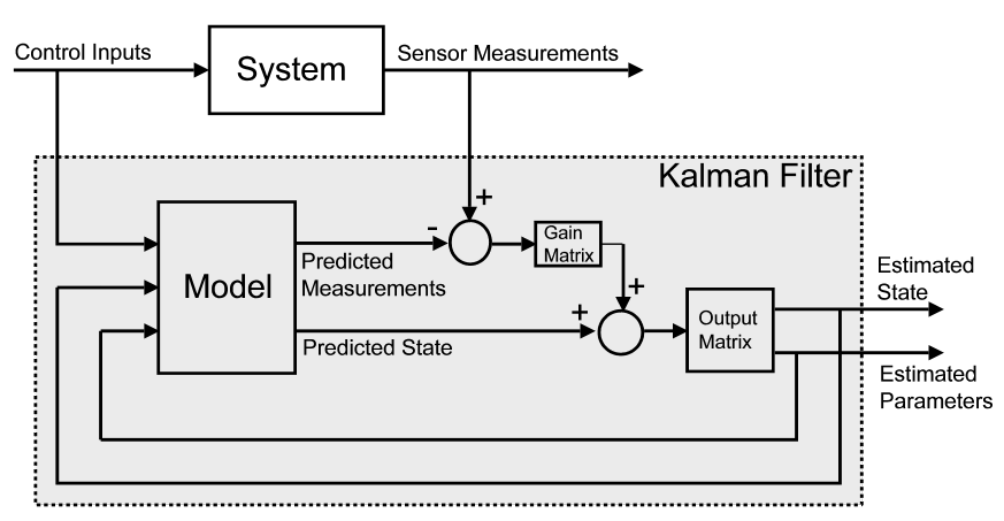
\includegraphics[scale=1]{images/kalman.png}
	\caption{Diagrama de blocos do filtro de Kalman. Fonte: Charles, G. \textit{et al.}, 2008.}
\end{figure}
\end{frame}

\begin{frame}{Funcionamento}
O artigo utiliza o filtro de Kalman da seguinte maneira:

\begin{itemize}
	\item os parâmetros mensurados no \textit{frame} são o centro de massa do objeto, seu deslocamento e a taxa de oclusão;
	\item o modelo assume que o movimento do objeto é uniforme, com velocidade constante;
	\item a taxa de oclusão também é utilizada para adaptar o modelo, tornando o filtro adaptativo.
\end{itemize}
\end{frame}

\section{Implementação}

%%%%%%%%%%%%%%%%%%%%%%%%%%%%%%%%%%%%%%%%%%%%%%%%%%%%%%%%%%%%%%%%%%%%%%%%%%%%%%%%
% Segmentação dos objetos de interesse
%%%%%%%%%%%%%%%%%%%%%%%%%%%%%%%%%%%%%%%%%%%%%%%%%%%%%%%%%%%%%%%%%%%%%%%%%%%%%%%%
\begin{frame}[fragile]{Seleção do objeto de interesse}
	A seleção do objeto de interesse é realizada manualmente pelo usuário, o qual define um ponto inicial com o auxílio de uma interface gráfica.
\end{frame}

\begin{frame}{Segmentação inicial do objeto}

	A partir da seleção do usuário no \textit{frame} $t$,  do objeto de interesse é segmentado através da diferença com os \textit{frames} $t-1$ e $t+1$, utilizando a equação (\ref{equ:fd}).
	
	\begin{equation}
	\label{equ:fd}
	FD(x, y, t) = 
	\begin{cases}
		0 \quad se\ \left| f(x, y, t + 1) - f(x, y, t) \right| \ \le \ T,\\
		1 \quad \text{caso contrário},
	\end{cases}
	\end{equation}

\end{frame}

\begin{frame}{Segmentação inicial do objeto}
	O objeto de interesse é definido como a interseção entre os dois valores de $FD$, conforme a equação (\ref{equ:mr}).
	\begin{equation}
		\label{equ:mr}
		MR(x, y) = FD(x, y, t-1) \cap FD(x, y, t)
	\end{equation}
	
	E a área do objeto de interesse é dada pela região onde os valores de MR é igual a 1, equação (\ref{equ:mrs}).
	\begin{equation}
		\label{equ:mrs}
		MRS(x, y) = \{(x,y) \ | \ MR(x,y,t) = 1\}
	\end{equation}
\end{frame}

\begin{frame}{Segmentação inicial do objeto}

	Um algoritmo de preenchimento de região morfológico é utilizado para separar um único objeto conectado, visto que o resultado de $MRS(x, y)$ pode conter mais de um objeto em movimento.

\end{frame}

\begin{frame}{Extração das características do objeto}

	Em seguida, o algoritmo \textit{K-means} é utilizado para determinar a cor dominante do objeto.
	
	Todo processamento posterior é realizado utilizando o modelo de cor HSI.

\end{frame}

\begin{frame}{Aplicação do filtro de Kalman adaptativo}
	\begin{figure}[H]
		\label{fig:flowchart}
		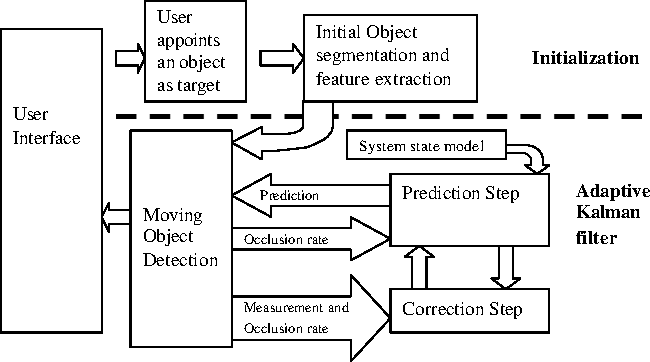
\includegraphics[scale=0.8]{images/flowchart.pdf}
		\caption{Fluxograma do sistema utilizando o filtro de Kalman adaptativo. Fonte: Weng, S. K. \textit{et al.}, 2016.}
	\end{figure}
\end{frame}

\section{Resultados}

%%%%%%%%%%%%%%%%%%%%%%%%%%%%%%%%%%%%%%%%%%%%%%%%%%%%%%%%%%%%%%%%%%%%%%%%%%%%%%%%
%Estimação do movimento com filtro de Kalman
%%%%%%%%%%%%%%%%%%%%%%%%%%%%%%%%%%%%%%%%%%%%%%%%%%%%%%%%%%%%%%%%%%%%%%%%%%%%%%%%
\begin{frame}{Resultados}
\begin{figure}[H]
	\label{fig:short}
	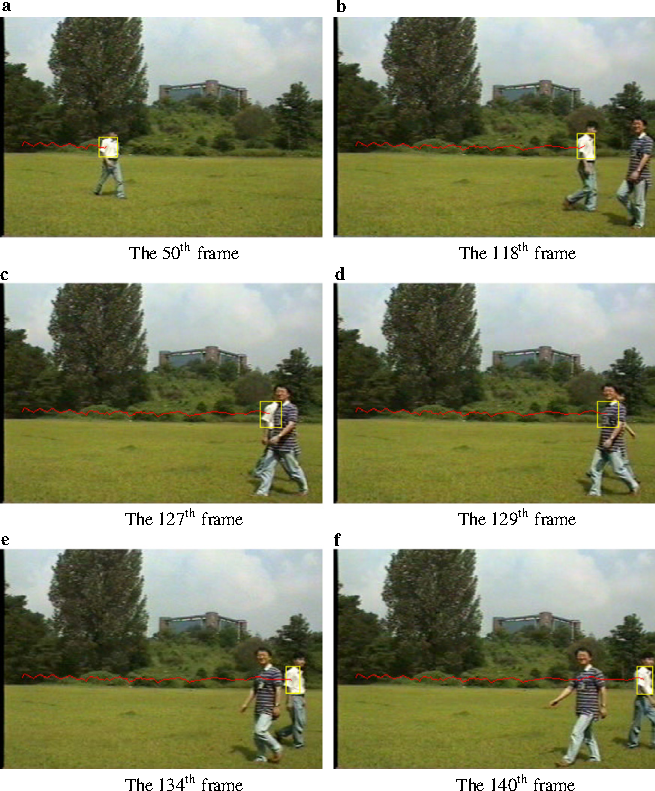
\includegraphics[scale=0.45]{images/result.pdf}
	\caption{Resultado do rastreamento com oclusão total de curta duração. Fonte: Weng, S. K. \textit{et al.}, 2016.}
\end{figure}
\end{frame}

\begin{frame}{Resultados}
\begin{figure}[H]
	\label{fig:long}
	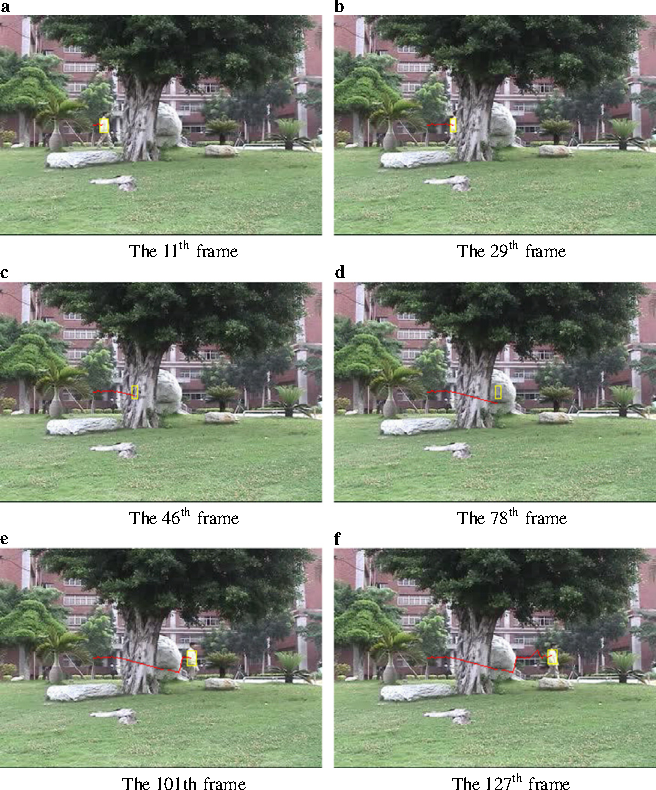
\includegraphics[scale=0.45]{images/result-long.pdf}
	\caption{Resultado do rastreamento com oclusão total de longa duração. Fonte: Weng, S. K. \textit{et al.}, 2016.}
\end{figure}
\end{frame}

\section{Conclusão}

\begin{frame}{Conclusão}
O artigo apresentou a aplicação efetiva de um filtro de Kalman adaptativo para o rastreamento de objetos em movimento.

Na abordagem proposta, a taxa de oclusão do objeto é utilizada para ajustar o modelo de movimento do filtro de modo adaptativo, proporcionando a capacidade de realizar o rastreamento mesmo com a oclusão total do objeto de interesse.

Segundo os resultados obtidos, o algoritmo pode ser utilizado em sistemas de tempo real.

\end{frame}

\begin{frame}[standout]
	Perguntas?
\end{frame}

\appendix

\begin{frame}[allowframebreaks]{Referências}

  \bibliography{apresentacao}
  \bibliographystyle{abbrv}

\end{frame}

\end{document}
